\documentclass{beamer}

\usepackage[utf8]{inputenc}
\usepackage{graphicx}
\usepackage{biblatex}

\title{Re-Encryption Mix-Net Module}
\author{Vitalis Salis}
\date{2017}

\begin{document}
    \frame{\titlepage}

    \begin{frame}
        \frametitle{Zeus}
        \begin{itemize}
            \item Web-based open-audit e-voting system.
            \item Open source.\footnote{\url{https://github.com/grnet/zeus}}
            \item Derived from Helios\footnote{
                \url{https://github.com/benadida/helios}
            }.
            \item Uses the Sako-Kilian re-encryption mix-net for anonymity.
            \item Already used by various institutions for elections.
        \end{itemize}
    \end{frame}

    \begin{frame}
        \begin{figure}
            \centering
            \includegraphics[width=12cm,height=7cm,keepaspectratio]{zeus-chart.eps}
            \caption{Registered and actual voters on Zeus.}
        \end{figure}
    \end{frame}

    \begin{frame}
        \frametitle{The Issue}
        \begin{itemize}
            \item The re-encryption mix-net used by Zeus is impractical.
            \item It requires a lot of costly, performance wise, cryptographic.
            operations, leading to longer times to get the election results.
            \item I.e for 10,000 votes the mixnet might take up to 8 hours!
            \item Our goal is to create an open source Python module that
            implements a faster re-encryption mix-net for applications
            requiring anonymity.
        \end{itemize}
    \end{frame}

    \begin{frame}
        \frametitle{Faster Mix-Nets}
        \begin{itemize}
            \item In order to overcome this issue, we've been looking on new
            research about mix-nets that guarantee faster performance.
            \item The best candidate we identified is proposed by Fauzi et al,
            from the University of Tartu.\footnote{
                \url{https://eprint.iacr.org/2016/866}
            }.
            \item The mix-net is based on elliptic curves.
        \end{itemize}
    \end{frame}

    \begin{frame}
        \frametitle{Existing Prototypes}
        \begin{itemize}
            \item A Python prototype that implements the mix-net proposed by
            Fauzi et al, was developed by GRNET\footnote{
                \url{https://github.com/grnet/ac16/}
            }.
            \item Still, the prototype wasn't satisfying.
            \item The main issue we identified was that multiplications on the
            elliptic curve structure are slow.
            \item The library implementing those multiplications is OpenSSL.
            \item A good replacement for OpenSSL is a similar library,
            libff.\footnote{\url{https://github.com/scipr-lab/libff}}
        \end{itemize}
    \end{frame}

    \begin{frame}
        \frametitle{Metrics}
        \begin{itemize}
            \item In order to compare these libraries we have defined specific 
            metrics.
            \item Our profiling involved a test case where we performed
            thousands of multiplications from C on both libraries:\newline
            $g ^ \rho$
            where $g$ is the generator of the elliptic curve group and
            $\rho$ is a 256 bit number.
            \item libff yielded up to 6 times better performance than OpenSSL.
            \item So, we moved forward with the implementation of a libff
            wrapper for Python.
        \end{itemize}
    \end{frame}

    \begin{frame}
        \frametitle{Wrapping libff With Cython}
        \begin{itemize}
            \item libff is implemented in C++.
            \item So it needs to be wrapped by Python in order to be used as a
            Python module.
            \item No such wrapper exists, so we set out to create one.
            \item We identified that Cython is the best candidate for wrapping
            libff.
            \item The wrapper exists as a separate open source module
            so it can be used by other Python projects that need to use libff.
        \end{itemize}
    \end{frame}

    \begin{frame}
        \frametitle{Comparing Wrappers}
        \begin{itemize}
            \item After creating the Cython wrapper for libff, in order to
            verify that it is indeed better than the Python wrapper for
            OpenSSL, we defined specific metrics.
            \item Our profiling involved a test case where we performed
            thousands of multiplications from Python on both wrappers.
            \item The results validated our hypothesis, so we'll use the Cython
            wrapper for the implementation of the re-encryption mix-net module.
        \end{itemize}
    \end{frame}

    \begin{frame}
        \frametitle{Future Work}
        \begin{itemize}
            \item Python Module
            \item Integration with Zeus
            \item Testing
        \end{itemize}
    \end{frame}
    \begin{frame}
        \center{\url{https://github.com/eellak/gsoc17module-zeus}}
    \end{frame}
\end{document}
